\section{Convolutional Neural Networks}

There are several types if neural networks, each designed to handle different types of data and tasks. Although neural networks might not always be the best choice for every problem, for instance, fully-connected-networks are not consistently better than random forests or SVM. However, for certain tasks, like image recognition, convolutional neural networks (CNNs) have shown remarkable performance.

\subsection{Convolutional Neural Networks (CNNs)}

\begin{definition}
    Consider a $K$-class classification problem with training data
    \[
        (\bm{y}^i, \bm{Z}^{1, i}), \quad i = 1, 2, \ldots, l
    \]
    where $\bm{y}^i \in \mathbb{R}^K$ is the label vector and $\bm{Z}^{1, i}$ is the input \red{image}.
\end{definition}

\vspace{1em}

If $\bm{Z}^{1, i}$ is in class $k$, then \[
    y^i = \left[\underbrace{0, \ldots, 0}_{k-1}, 1, 0, \ldots, 0 \right]^T \in \mathbb{R}^K
\]
CNN can map the input image $\bm{Z}^{1, i}$ to the label vector $\bm{y}^i$. Typically, CNN consists of several convolutional layers followed by fully-connected layers.

\newpage

\subsection{Convolutional Layer}

The input and output of a convolutional layer are assume to be \red{images}.  
\begin{definition}
    For a single convolutional layer, the input image is denoted as
    \[
        \bm{Z}^{\text{in}}: a^{\text{in}} \times b^{\text{in}} \times d^{\text{in}}
    \]
    where $a^{\text{in}}$ and $b^{\text{in}}$ are the height and width of the image, and $d^{\text{in}}$ is the number of channels (e.g., 3 for RGB images).
\end{definition}

\begin{figure}[H]
    \centering
    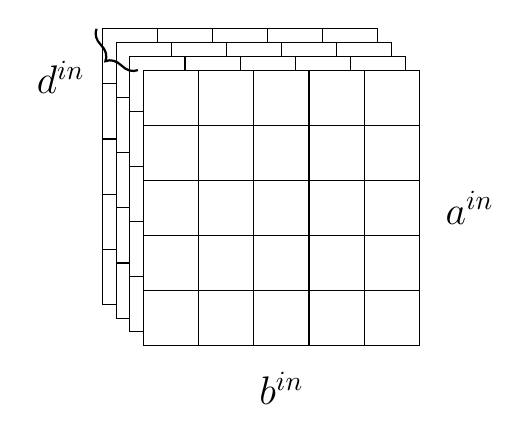
\begin{tikzpicture}[
        grid line/.style={black, thin},
        border line/.style={black},
        box fill/.style={fill=white},
        label text/.style={font=\Large},
        scale=0.7
    ]

        \def\gridW{5}
        \def\gridH{5}
        \def\depth{3}
        \def\xoffset{-0.25}
        \def\yoffset{0.25}

        \foreach \z in {\depth, ..., 0} {
            \begin{scope}[shift={(\z*\xoffset, \z*\yoffset)}]
                \fill[box fill] (0,0) rectangle (\gridW, \gridH);
                \draw[grid line, step=1] (0,0) grid (\gridW, \gridH);
                \draw[border line] (0,0) rectangle (\gridW, \gridH);
            \end{scope}
        }

        \node[label text, anchor=west] at (\gridW + 0.3, \gridH/2) {$a^{\text{in}}$};
        \node[label text, anchor=north] at (\gridW/2, -0.3) {$b^{\text{in}}$};

        \coordinate (BackTopLeft) at (\depth*\xoffset, \gridH + \depth*\yoffset);
        \coordinate (FrontTopLeft) at (0, \gridH);

        % 修改 2: 改用標準 "brace"
        % 拿掉了 "calligraphic" 關鍵字
        \draw[decorate, decoration={brace, amplitude=6pt, mirror}, thick] 
            ([xshift=-3pt]BackTopLeft) -- ([xshift=-3pt]FrontTopLeft)
            node[midway, left=8pt, label text, yshift=-10pt] {$d^{\text{in}}$};

    \end{tikzpicture}
    \caption{Input of a convolutional layer}
\end{figure}

The goal is to generate an output image \[
    \bm{Z}^{\text{out}, i}: a^{\text{out}} \times b^{\text{out}} \times d^{\text{out}}
\]
Consider a set of $d^{\text{out}}$ filters (or kernels), filter $j \in \{1, \ldots, d^{\text{out}}\}$ has dimensions \[
    h \times h \times d^{\text{in}}
\]
\[
    \begin{pmatrix}
        w^{j}_{1,1,1} & \cdots & w^{j}_{1,h,1} \\
        \vdots & \ddots & \vdots \\
        w^{j}_{h,1,1} & \cdots & w^{j}_{h,h,1}
    \end{pmatrix}, \cdots,
    \begin{pmatrix}
        w^{j}_{1,1,d^{\text{in}}} & \cdots & w^{j}_{1,h,d^{\text{in}}} \\
        \vdots & \ddots & \vdots \\
        w^{j}_{h,1,d^{\text{in}}} & \cdots & w^{j}_{h,h,d^{\text{in}}}
    \end{pmatrix}
\]
where $h$ is the filter size (height and width, layer index is omitted for simplicity)

\definecolor{customblue}{RGB}{60, 120, 230}

\begin{figure}[H]
    \centering

    \begin{tikzpicture}[
        basic grid/.style={black, thin},
        box fill/.style={fill=white},
        % 藍色高亮 (實線) - 用於最前面
        highlight solid/.style={customblue, ultra thick},
        % 藍色高亮 (虛線) - 用於深度透視
        highlight dashed/.style={customblue, very thick, dashed},
        % 連接線
        connector line/.style={customblue, thin},
        input label/.style={font=\tiny, color=customblue, align=center},
        output label/.style={align=center}
    ]
    
        % --- 參數設定 ---
        \def\gridW{5}
        \def\gridH{5}
        \def\depth{3}
        \def\kernelSize{3}
        
        % 透視偏移量
        \def\xoffset{-0.1}
        \def\yoffset{0.1}
    
        % =========================================
        % 1. 繪製左側輸入體積 (Input Volume)
        % =========================================
        % 修正點:移除 \depth-1 的運算,直接寫 {\depth, ..., 0}
        \foreach \z in {\depth, ..., 0} {
            \begin{scope}[shift={(\z*\xoffset, \z*\yoffset)}]
                \fill[box fill] (0, 0) rectangle (\gridW, \gridH);
                \draw[basic grid] (0, 0) grid (\gridW, \gridH);
                \draw[black] (0, 0) rectangle (\gridW, \gridH); % 加強外框
            \end{scope}
        }
    
        % =========================================
        % 2. 繪製卷積核 (Kernel Window)
        % =========================================
        % 我們設定卷積核在左上角 (0, 0) 到 (3, 3) 的位置
        % 注意:在 TikZ 座標中,(0, gridH) 是左上角
        
        % 定義關鍵座標
        % 前面層 (z=0) 的左上與右下
        \coordinate (Front_TL) at (0, \gridH - 1);
        \coordinate (Front_BR) at (\kernelSize, \gridH-\kernelSize-1);
        \coordinate (Front_TR) at (\kernelSize, \gridH - 1);
        \coordinate (Front_BL) at (0, \gridH-\kernelSize - 1);
    
        % 背面層 (z=depth) 的偏移量
        \coordinate (BackShift) at (\depth*\xoffset, \depth*\yoffset);
        
        % 背面層對應的四個角
        \coordinate (Back_TL) at ($(Front_TL) + (BackShift)$);
        \coordinate (Back_TR) at ($(Front_TR) + (BackShift)$);
        \coordinate (Back_BL) at ($(Front_BL) + (BackShift)$);
        \coordinate (Back_BR) at ($(Front_BR) + (BackShift)$);
    
        \coordinate (Front_TLs) at (0, \gridH);
        \coordinate (Front_BRs) at (\kernelSize, \gridH-\kernelSize);
        \coordinate (Front_TRs) at (\kernelSize, \gridH);
        \coordinate (Front_BLs) at (0, \gridH-\kernelSize);
    
        \coordinate (Back_TLs) at ($(Front_TLs) + (BackShift)$);
        \coordinate (Back_TRs) at ($(Front_TRs) + (BackShift)$);
        \coordinate (Back_BLs) at ($(Front_BLs) + (BackShift)$);
        \coordinate (Back_BRs) at ($(Front_BRs) + (BackShift)$);
    
        % 2.1.5 畫深度連接線 (虛線)
        \draw[highlight dashed] (Front_TLs) -- (Back_TLs);
        \draw[highlight dashed] (Front_TRs) -- (Back_TRs);
        \draw[highlight dashed] (Front_BLs) -- (Back_BLs);
        \draw[highlight dashed] (Front_BRs) -- (Back_BRs);
    
        % 2.2.5 畫背面框 (虛線)
        \draw[highlight dashed] (Back_TLs) -- (Back_TRs) -- (Back_BRs) -- (Back_BLs) -- cycle;
    
        % 2.3 畫前面框 (實線) - 這要最後畫才不會被遮住
        \draw[highlight dashed] (Front_TLs) rectangle (Front_BRs);
    
        % 背面層 (z=depth) 的偏移量
        \coordinate (BackShift) at (\depth*\xoffset, \depth*\yoffset);
        
        % 背面層對應的四個角
        
    
        % 2.1 畫深度連接線 (虛線)
        \draw[highlight solid] (Front_TL) -- (Back_TL);
        \draw[highlight solid] (Front_TR) -- (Back_TR);
        \draw[highlight solid] (Front_BL) -- (Back_BL);
        \draw[highlight solid] (Front_BR) -- (Back_BR);
    
        % 2.2 畫背面框 (虛線)
        \draw[highlight solid] (Back_TL) -- (Back_TR) -- (Back_BR) -- (Back_BL) -- cycle;
    
        % 2.3 畫前面框 (實線) - 這要最後畫才不會被遮住
        \draw[highlight solid] (Front_TL) rectangle (Front_BR);
    
        % 2.4 填寫輸入層的小數字 (i,j,1)
        \foreach \i [count=\iy from 0] in {1,2,3} { 
            \foreach \j [count=\jx from 0] in {1,2,3} { 
                % 座標計算:x = j-0.5, y = gridH - (i-0.5)
                \node[input label] at (\jx + 0.5, \gridH - \iy - 1.5) {\i,\j,1};
            }
        }
    
        % 繪製向下的大藍色箭頭 (指示滑動方向)
        \draw[-{Triangle[width=10pt, length=10pt]}, customblue, line width=3pt] 
            (\kernelSize/2, \gridH) -- (\kernelSize/2, \kernelSize + 1.0);
    
        % =========================================
        % 3. 繪製右側輸出 (Output Map)
        % =========================================
        \begin{scope}[shift={(\gridW + 4, \gridH - 3)}]
            \def\outSize{2} % 顯示 2x2 的輸出示意
            
            % 3.1 畫格子
            \fill[box fill] (0,0) rectangle (\outSize, \outSize);
            \draw[basic grid] (0,0) grid (\outSize, \outSize);
            \draw[black] (0,0) rectangle (\outSize, \outSize);
            
            % 3.2 高亮對應的輸出格 (左上角)
            \draw[highlight solid] (0, 1-1) rectangle (1, 2-1);
            
            % 輸出格的四個角 (用於連接)
            \coordinate (Out_TL) at (0, 2-1);
            \coordinate (Out_TR) at (1, 2-1);
            \coordinate (Out_BL) at (0, 1-1);
            \coordinate (Out_BR) at (1, 1-1);
    
            % 3.3 文字標籤
            \node[output label] at (0.5, 1.5) {$\boldsymbol{s_{1,1,j}^{\text{out},i}}$};
            \node[output label] at (1.5, 1.5) {$\boldsymbol{s_{1,2,j}^{\text{out},i}}$};
            \node[output label] at (0.5, 0.5) {$\boldsymbol{s_{2,1,j}^{\text{out},i}}$};
            \node[output label] at (1.5, 0.5) {$\boldsymbol{s_{2,2,j}^{\text{out},i}}$};
        \end{scope}
    
        % =========================================
        % 4. 繪製中間的投影連接線
        % =========================================
        % 這裡從前面的框 (Front) 連到輸出框 (Out)
        \draw[connector line] (Front_TR) -- (Out_TR);
        \draw[connector line] (Front_BR) -- (Out_BR);
        \draw[connector line] (Front_BL) -- (Out_BL);
        \draw[connector line] (Front_TL) -- (Out_TL);
        
        % 為了視覺效果,這些線通常畫在最上層,或者根據需要調整
    \end{tikzpicture}
    \caption{Convolutional Layer Illustration}
\end{figure}

\newpage

To compute the $j$-th channel of the output image, we scan the input from top-left to bottom-right. At each position obtain the sub-image \[
    \bm{S}^{\text{in}}: h \times h \times d^{\text{in}}
\]
We calculate the inner product between each sub-image and the $j$-th filter to get a single scalar value \[
    s_{u,v,j}^{\text{out}, i} = \langle \bm{S}^{\text{in}}, \bm{W}^j \rangle
\]
The idea of doing this operation is to extract local features from the input image. For instance, edges, corners, and textures can be detected by appropriate filters. If we start from the top-left corner of the input image, the first sub-image of channel $d$ is \[
    \bm{S}^{i}_{1,1,d} = 
    \begin{pmatrix}
        z^{i}_{1,1,d} & \cdots & z^{i}_{1,h,d} \\
        \vdots & \ddots & \vdots \\
        z^{i}_{h,1,d} & \cdots & z^{i}_{h,h,d}
    \end{pmatrix}
\]
We then calculate \[
    s_{1,1,j}^{\text{out}, i} = \sum_{d=1}^{d^{\text{in}}} \left\langle \begin{pmatrix}
        z^{i}_{1,1,d} & \cdots & z^{i}_{1,h,d} \\
        \vdots & \ddots & \vdots \\
        z^{i}_{h,1,d} & \cdots & z^{i}_{h,h,d}
    \end{pmatrix}, \begin{pmatrix}
        w^{j}_{1,1,d} & \cdots & w^{j}_{1,h,d} \\
        \vdots & \ddots & \vdots \\
        w^{j}_{h,1,d} & \cdots & w^{j}_{h,h,d}
    \end{pmatrix} \right\rangle + b_j \tag{1}
\]
where $\langle \cdot, \cdot \rangle$ denotes the component-wise inner product between two matrices. This value becomes the $(1,1)$ position of the $j$-th channel of the output image. Next, we use other sub-images to compute other positions of the output image. Let the stride $s$ be the number of pixels vertically or horizontally to get the next sub-image. For the position $(2, 1)$, we move vertically down by $s$ pixels to get the sub-image \[
    \bm{S}^{i}_{2,1,d} =
    \begin{pmatrix}
        z^{i}_{1+s,1,d} & \cdots & z^{i}_{1+s,h,d} \\
        \vdots & \ddots & \vdots \\
        z^{i}_{h+s,1,d} & \cdots & z^{i}_{h+s,h,d}
    \end{pmatrix}
\]
Then we can get $(2,1)$ position of the $j$-th channel of the output image by \[
    s_{2,1,j}^{\text{out}, i} = \sum_{d=1}^{d^{\text{in}}} \left\langle \begin{pmatrix}
        z^{i}_{1+s,1,d} & \cdots & z^{i}_{1+s,h,d} \\
        \vdots & \ddots & \vdots \\
        z^{i}_{h+s,1,d} & \cdots & z^{i}_{h+s,h,d}
    \end{pmatrix}, \begin{pmatrix}
        w^{j}_{1,1,d} & \cdots & w^{j}_{1,h,d} \\
        \vdots & \ddots & \vdots \\
        w^{j}_{h,1,d} & \cdots & w^{j}_{h,h,d}
    \end{pmatrix} \right\rangle + b_j \tag{2}
\]

\begin{theorem}
    The output image size can be calculated respectively by \[
        a^{\text{out}} = \left\lfloor \frac{a^{\text{in}} - h}{s} \right\rfloor + 1, \quad b^{\text{out}} = \left\lfloor \frac{b^{\text{in}} - h}{s} \right\rfloor + 1 \tag{3}
    \]
\end{theorem}
\begin{proof}
    Vertically, the last valid starting position for the sub-image is at row \[
        h, h+s, h+2s, \ldots, h + \Delta s \leq a^{\text{in}}
    \]
    Thus, we have \[
        h + \Delta s \leq a^{\text{in}} \implies \Delta \leq \frac{a^{\text{in}} - h}{s}
    \]
    Hence, $\displaystyle \Delta = \left\lfloor \frac{a^{\text{in}} - h}{s} \right\rfloor$
\end{proof}

\newpage

\subsection{Matrix Operations}

To implement convolutional layers efficiently, we should use the matrix-matrix and matrix-vector operations to do the convalutional operation (simplify the optimization). We first collect images of all channels as the input matrix \[
    \bm{Z}^{\text{in}, i} =
    \begin{pmatrix}
        z^{i}_{1,1,1} & z^{i}_{2,1,1} & \cdots & z^{i}_{a^{\text{in}},b^{\text{in}},1} \\
        \vdots & \vdots & \ddots & \vdots \\
        z^{i}_{1,1,d^{\text{in}}} & z^{i}_{2,1,d^{\text{in}}} & \cdots & z^{i}_{a^{\text{in}},b^{\text{in}},d^{\text{in}}}
    \end{pmatrix} \in \mathbb{R}^{d^{\text{in}} \times (a^{\text{in}} b^{\text{in}})}
\]
and let all filters to be \[
    W = \begin{pmatrix}
        w^{1}_{1,1,1} & w^{2}_{1,1,1} & \cdots & w^{d^{\text{out}}}_{1,1,1} \\
        \vdots & \vdots & \ddots & \vdots \\
        w^{1}_{h,h,d^{\text{in}}} & w^{2}_{h,h,d^{\text{in}}} & \cdots & w^{d^{\text{out}}}_{h,h,d^{\text{in}}}
    \end{pmatrix}
    \in \mathbb{R}^{(h h d^{\text{in}}) \times d^{\text{out}}}
\]
by the parameters of current layer. The bias vector is \[
    b = \begin{pmatrix}
        b_1 \\ b_2 \\ \vdots \\ b_{d^{\text{out}}}
    \end{pmatrix} \in \mathbb{R}^{d^{\text{out}}}
\]
Then we get 
\begin{definition}
    The operation of a single convolutional layer as \[
        \bm{S}^{\text{out}, i} = W \phi(\bm{Z}^{\text{in}, i}) + b \mathbbm{1}^T_{a^{\text{out}} b^{\text{out}}} \tag{1.1}
    \]
\end{definition}
where \[
    \mathbbm{1}_{a^{\text{out}} b^{\text{out}}} = \begin{pmatrix}
        1 \\ 1 \\ \vdots \\ 1
    \end{pmatrix} \in \mathbb{R}^{a^{\text{out}} b^{\text{out}} \times 1}
\]
and $\phi(\bm{Z}^{\text{in}, i})$ collects all sub-images in $\bm{Z}^{\text{in}, i}$ as columns. Specifically, the \[
    \phi(\bm{Z}^{\text{in}, i}) =
    \begin{pmatrix}
        z^{i}_{1,1,1} & z^{i}_{1+s,1,1} & \cdots & z^{i}_{1+(a^{\text{out}}-1)s, 1+(b^{\text{out}}-1)s,1} \\
        z^{i}_{2,1,1} & z^{i}_{2+s,1,1} & \cdots & z^{i}_{2+(a^{\text{out}}-1)s, 1+(b^{\text{out}}-1)s,1} \\
        \vdots & \vdots & \ddots & \vdots \\
        z^{i}_{h,h,1} & z^{i}_{h+s,h+s,1} & \cdots & z^{i}_{h+(a^{\text{out}}-1)s, h+(b^{\text{out}}-1)s,1} \\
        \vdots & \vdots & \ddots & \vdots \\
        z^{i}_{h,h,d^{\text{in}}} & z^{i}_{h+s,h+s,d^{\text{in}}} & \cdots & z^{i}_{h+(a^{\text{out}}-1)s, h+(b^{\text{out}}-1)s,d^{\text{in}}}
    \end{pmatrix} \in \mathbb{R}^{(h h d^{\text{in}}) \times (a^{\text{out}} b^{\text{out}})}
\]
Next we consider the activation function scales each element of $\bm{S}^{\text{out}, i}$ to obtain the output matrix \[
    \bm{Z}^{\text{out}, i} = \sigma(\bm{S}^{\text{out}, i}) \in \mathbb{R}^{d^{\text{out}} \times (a^{\text{out}} b^{\text{out}})} \tag{1.2}
\]
For CNN, we usually use ReLU as the activation function.
\[
    \sigma(x) = \max(0, x) \tag{1.3}
\]
We need it to be differentiable for backpropagation, but ReLU is not differentiable at $x=0$. In practice, (Krizhevsky et al.) we can define \[
    \sigma'(x) = \begin{cases}
        1 &\text{if } x > 0 \\
        0 &\text{otherwise}
    \end{cases}
\]

In the matrix-matrix product form \[
    W \phi(\bm{Z}^{\text{in}, i})
\]
each element is the inner product between a filter and a sub-image. Clearly, $\phi$ is a linear mapping from $\mathbb{R}^{d^{\text{in}} \times (a^{\text{in}} b^{\text{in}})}$ to $\mathbb{R}^{(h h d^{\text{in}}) \times (a^{\text{out}} b^{\text{out}})}$, so there exists a matrix $P_{\phi}$ such that

\begin{definition*}
    For the linear mapping $\phi$, we have
    \begin{definition}[Convolutional Mapping]
        \[
            \phi(\bm{Z}^{\text{in}, i}) = \text{mat}\left( P_{\phi} \, \text{vec}(\bm{Z}^{\text{in}, i}) \right)_{(h h d^{\text{in}}) \times (a^{\text{out}} b^{\text{out}})},\ \forall i \tag{1.4}
        \]
    \end{definition}
    \begin{definition}[Vectorization]
        For a matrix $M$'s columns concatenated to a vector $\mathbf{v}$ \[
            \text{vec}(M) = \mathbf{v} = \begin{pmatrix}
                M_{:,1} \\
                M_{:,2} \\
                \vdots \\
                M_{:,n}
            \end{pmatrix} \in \mathbb{R}^{ab \times 1}, \quad \text{where } M \in \mathbb{R}^{a \times b}
        \]
    \end{definition}
    \begin{definition}[Matrix Reshaping]
        $\text{mat}(\mathbf{v})$ is the inverse operation of $\text{vec}(M)$, which reshapes the vector $\mathbf{v} \in \mathbb{R}^{ab \times 1}$ back to the matrix $M \in \mathbb{R}^{a \times b}$ \[
            \text{mat}(\mathbf{v}_{ab \times 1})_{a \times b} = M = \begin{pmatrix}
                v_{1} & v_{a+1} & \cdots & v_{(b-1)a+1} \\
                v_{2} & v_{a+2} & \cdots & v_{(b-1)a+2} \\
                \vdots & \vdots & \ddots & \vdots \\
                v_{a} & v_{2a} & \cdots & v_{ba}
            \end{pmatrix} \in \mathbb{R}^{a \times b}
        \]
    \end{definition}
    \begin{definition}
        $P_{\phi}$ is a huge sparse matrix \[
            P_{\phi} \in \mathbb{R}^{(h h d^{\text{in}})(a^{\text{out}} b^{\text{out}}) \times d^{\text{in}} (a^{\text{in}} b^{\text{in}})}
        \] and 
        \[
            \phi : \mathbb{R}^{d^{\text{in}} \times (a^{\text{in}} b^{\text{in}})} \to \mathbb{R}^{(h h d^{\text{in}}) \times (a^{\text{out}} b^{\text{out}})}
        \]
    \end{definition}
\end{definition*}

\begin{remark}
    $P_{\phi}$ 是用來做區塊提取的 (Patch Extraction Matrix), 將 $\text{vec}(Z^{\text{in}, i})$ 裡面所有 sub-image 提取出來,最後再經過 mat() 變回矩陣形式,這樣就可以讓卷積運算變成矩陣乘法 \[
        W \phi(\bm{Z}^{\text{in}, i}) + b \mathbbm{1}^T_{a^{\text{out}} b^{\text{out}}}
    \]
    並且,使用 $P_{\phi}$ 的好處是可以很方便地計算反向傳播的梯度,因為 $P_{\phi}$ 是 Linear Mapping,可以直接利用矩陣微積分的規則來計算梯度,直接 Chain Rule 就可以了 \[
        \frac{\partial \xi}{\partial\, \text{vec}(\bm{Z}^{\text{in}, i})} = P_{\phi}^T \frac{\partial \xi}{\partial\, \text{vec}(\phi(\bm{Z}^{\text{in}, i}))}
    \]
\end{remark}

\subsection{Optimization Problem for CNN}

We collect all parameters of the convolutional layer as \[
    \theta = \begin{pmatrix}
        \text{vec}(W^1) \\
        \bm{b}^1 \\
        \vdots \\
        \text{vec}(W^L) \\
        \bm{b}^L 
    \end{pmatrix} \in \mathbb{R}^n, \quad \text{where } n = \# \ \text{total parameters}
\]
The output of last layer $L$ is vector $\bm{z}^{L+1, i} (\theta)$. Consider the loss function such as squared loss \[
    \xi_i(\theta) = \|\bm{y}^i - \bm{z}^{L+1, i}(\theta)\|^2_2
\]
\begin{definition}
    The overall optimization problem for CNN is \[
        \min_{\theta} f(\theta)    
    \]
    where \[
        f(\theta) = \frac{1}{2C} \theta^T \theta + \frac{1}{l} \sum_{i=1}^{l} \xi(z^{L+1, i}(\theta); \bm{y}^i, \bm{Z}^{1, i})
    \]
\end{definition}
where $C > 0$ is the regularization parameter, which is same as the fully-connected networks.

\begin{note}
    We devide the sum of loss by $l$ to get the average loss per sample. 這樣做的好處是當我們改變訓練資料的大小 $l$ 時,不需要重新調整 learning rate,因為 average loss 已經把資料數量的影響給 normalize 掉了。
\end{note}

\subsection{Padding Layers}
Besides convolutional layers, CNNs often include other operations such as pooling layers and padding layers.

First, we discuss padding layers. To better control the output size of convolutional layers, before the convolution operation, we can enlarge the input image by adding extra 0 around the border. This is called \textbf{zero padding}.

\begin{figure}[H]
    \centering

    \resizebox{0.35\textwidth}{!}{
    \begin{tikzpicture}[
        % 設定樣式
        zero text/.style={font=\Large},
        dot text/.style={font=\Large},
        brace style/.style={decorate, decoration={brace, amplitude=6pt}, thick},
        brace mirror style/.style={decorate, decoration={brace, amplitude=6pt, mirror}, thick},
        label text/.style={font=\large}, 
    ]
    
        % 1. 繪製中間的輸入圖片 (矩形)
        \node[draw, minimum width=2cm, minimum height=2cm, align=center, font=\sffamily] (image) at (0,0) {An input\\image};
    
        % 定義圖片的邊界座標 (方便後續定位)
        \coordinate (TL) at ($(image.north west)$); % Top Left
        \coordinate (TR) at ($(image.north east)$); % Top Right
        \coordinate (BL) at ($(image.south west)$); % Bottom Left
        \coordinate (BR) at ($(image.south east)$); % Bottom Right
    
        % 2. 繪製四個角落的 0 區塊 (Padding Corners)
        % 設定偏移距離
        \def\gap{0.8cm}
        \def\padW{1.2cm} % 0...0 的寬度估計
    
        % --- 左上角 (Top-Left) ---
        % 這裡由三行組成: 0..0, 垂直點, 0..0
        \node[zero text, above left=\gap and \gap of TL, anchor=south east] (tl_zeros_bottom) {$0 \cdots 0$};
        \node[dot text, above=0.1cm of tl_zeros_bottom] (tl_dots) {$\vdots$};
        \node[zero text, above=0.1cm of tl_dots] (tl_zeros_top) {$0 \cdots 0$};
    
        % --- 右上角 (Top-Right) ---
        \node[zero text, above right=\gap and \gap of TR, anchor=south west] (tr_zeros_bottom) {$0 \cdots 0$};
        \node[dot text, above=0.1cm of tr_zeros_bottom] (tr_dots) {$\vdots$};
        \node[zero text, above=0.1cm of tr_dots] (tr_zeros_top) {$0 \cdots 0$};
    
        % --- 左下角 (Bottom-Left) ---
        \node[zero text, below left=\gap and \gap of BL, anchor=north east] (bl_zeros_top) {$0 \cdots 0$};
        \node[dot text, below=0.1cm of bl_zeros_top] (bl_dots) {$\vdots$};
        \node[zero text, below=0.1cm of bl_dots] (bl_zeros_bot) {$0 \cdots 0$};
    
        % --- 右下角 (Bottom-Right) ---
        \node[zero text, below right=\gap and \gap of BR, anchor=north west] (br_zeros_top) {$0 \cdots 0$};
        \node[dot text, below=0.1cm of br_zeros_top] (br_dots) {$\vdots$};
        \node[zero text, below=0.1cm of br_dots] (br_zeros_bot) {$0 \cdots 0$};
    
    
        % 3. 繪製中間連接的點點 (Dots)
        % 上方中間
        \node[dot text] at ($(tl_zeros_bottom)!0.5!(tr_zeros_top)$) {$\cdots$};
        % 下方中間
        \node[dot text] at ($(bl_zeros_top)!0.5!(br_zeros_top) - (0, 1)$) {$\cdots$};
        % 左側中間
        \node[dot text] at ($(tl_zeros_bottom)!0.5!(bl_zeros_top)$) {$\vdots$};
        % 右側中間
        \node[dot text] at ($(tr_zeros_bottom)!0.5!(br_zeros_top)$) {$\vdots$};
    
        % 4. 繪製大括號與標籤 (Braces & Labels)
        
        % (a) 左上角的 p (水平)
        \draw[brace style] 
            ([yshift=5pt]tl_zeros_top.north west) -- ([yshift=5pt]tl_zeros_top.north east)
            node[midway, above=8pt, label text] {$p$};
    
        % (b) 左上角的 p (垂直)
        \draw[brace mirror style] 
            ([xshift=-5pt]tl_zeros_top.north west) -- ([xshift=-5pt]tl_zeros_bottom.south west)
            node[midway, left=8pt, label text] {$p$};
    
        % (c) 中間圖片寬度 a^in
        \draw[brace style] 
            ([yshift=2pt]TL) -- ([yshift=2pt]TR)
            node[midway, above=8pt, label text] {$a^{\text{in}}$};
    
        % (d) 中間圖片高度 b^in
        \draw[brace style] 
            ([xshift=2pt]TR) -- ([xshift=2pt]BR)
            node[midway, right=8pt, label text] {$b^{\text{in}}$};
    
    \end{tikzpicture}
    }
    \caption{Zero Padding Layer Illustration}
\end{figure}

The size of the input image will increase from \[
    a^{\text{in}} \times b^{\text{in}} \to (a^{\text{in}} + 2p) \times (b^{\text{in}} + 2p)
\]
The operation can be treated as a layer of mapping an input $\bm{Z}^{\text{in}, i}$ to an output $\bm{Z}^{\text{out}, i}$. 
\begin{definition}[Padding Layer]
    Assume that $d^{\text{in}} = d^{\text{out}}$ for all input, there must exist a $0/1$ matrix $P_{\text{pad}} \in \mathbb{R}^{d^{\text{out}} a^{\text{out}} b^{\text{out}} \times d^{\text{in}} a^{\text{in}} b^{\text{in}}}$ such that \[
        \bm{Z}^{\text{out}, i} \equiv \text{mat}\left( P_{\text{pad}} \, \text{vec}(\bm{Z}^{\text{in}, i}) \right)_{d^{\text{out}} \times (a^{\text{out}} b^{\text{out}})}
    \]
\end{definition}

\subsection{Pooling Layers}

In practice, after convolutional layers, we often get very large output images which will increase the computational cost of the following layers. To reduce the cost, we can use pooling layers to down-sample the output images or do the approximation that can extract the main (invariant) rotation/translation features of the images. There are many types of pooling layers, such as max pooling, average pooling, and stochatic pooling. Here we only discuss max pooling.

\begin{eg}
    Here is an example of max pooling layer with pool size $2 \times 2$ and stride $2$.
    \[
        \text{image A}: \quad
        \left(
        \begin{array}{cc|cc}
            2 & 3 & 6 & 8 \\
            \boxed{5} & 4 & \boxed{9} & 7 \\
            \hline
            1 & 2 & \boxed{6} & 0 \\
            \boxed{4} & 3 & 2 & 1
        \end{array}
        \right)
        \quad \xrightarrow[\text{pool size }2 \times 2, s=2]{\text{max pooling}} \quad
        \begin{pmatrix}
            5 & 9 \\
            4 & 6
        \end{pmatrix}
    \]
    \[
        \text{image B}: \quad
        \left(
        \begin{array}{cc|cc}
            3 & 2 & 3 & 6 \\
            4 & \boxed{5} & 4 & \boxed{9} \\
            \hline
            2 & 1 & 2 & \boxed{6} \\
            3 & \boxed{4} & 3 & 2
        \end{array}
        \right)
        \quad \xrightarrow[\text{pool size }2 \times 2, s=2]{\text{max pooling}} \quad
        \begin{pmatrix}
            5 & 9 \\
            4 & 6
        \end{pmatrix}
    \]
\end{eg}

In this example, $B$ is a translation horizontally for one pixel of $A$, we split the image into four $2 \times 2$ sub-images and take the maximum value of each sub-image as the output. In each sub-image, only some elements are changed, so the output maximum remains the same or similar, which is called \textbf{translation invariance}.

For the mathematical representation of max pooling layer, it can be treated as a mapping from input matrix $\bm{Z}^{\text{in}, i}$ to output matrix $\bm{Z}^{\text{out}, i}$. We can partition every channel of $\bm{Z}^{\text{in}, i}$ into non-overlapping sub-matrices by $h \times h$ filters with stride $s = h$.

By the same idea of convolutional layers, we can generate a huge sparse matrix \[
    \phi (\bm{Z}^{\text{in}, i}) = \text{mat}\left( P_{\phi} \, \text{vec}(\bm{Z}^{\text{in}, i}) \right)_{h h  \times d^{\text{in}} a^{\text{out}} b^{\text{out}}} \tag{1.5}
\]
where \[
    a^{\text{out}} = \left\lfloor \frac{a^{\text{in}} - h}{s} \right\rfloor + 1 = \left\lfloor \frac{a^{\text{in}}}{h} \right\rfloor, \quad b^{\text{out}} = \left\lfloor \frac{b^\text{in}}{h} \right\rfloor, \quad d^{\text{out}} = d^{\text{in}}
\]
Note that we now consider $hh \times d^{\text{out}} a^{\text{out}} b^{\text{out}}$ but not $hh d^{\text{out}} \times a^{\text{out}} b^{\text{out}}$ because can then do the max operation channel by channel. To select the maximum value from each sub-image, there exists a 0/1 matrix $M^i \in \mathbb{R}^{d^{\text{out}} a^{\text{out}} b^{\text{out}} \times h h d^{\text{out}} a^{\text{out}} b^{\text{out}}}$ so that each row of $M^i$ has only one 1 corresponding to the maximum value's position from $\text{vec}(\phi (\bm{Z}^{\text{in}, i}))$. Therefore, we have
\[
    \bm{Z}^{\text{out}, i} = \text{mat}\left( M^i \, \text{vec}(\phi (\bm{Z}^{\text{in}, i})) \right)_{d^{\text{out}} \times (a^{\text{out}} b^{\text{out}})} \tag{1.6}
\]

\begin{note}
    A comparison between convolutional layer and pooling layer is shown below
    \[
        \bm{S}^{\text{out}, i} = W \phi(\bm{Z}^{\text{in}, i}) + \bm{b} \mathbbm{1}^T_{a^{\text{out}} b^{\text{out}}}
    \]
    $M^i$ is a similar role as $W$ in convolutional layers, while $M^i$ is 0/1, which is not a constant, it is positions of 1's depend on the value of $\phi(\bm{Z}^{\text{in}, i})$.
\end{note}

By combining (1.5) and (1.6), we have

\begin{definition}[Max Pooling Layer]
    \[
        \bm{Z}^{\text{out}, i} = \text{mat}\left( P_{\text{pool}}^i \, \text{vec}(\bm{Z}^{\text{in}, i}) \right)_{d^{\text{out}} \times (a^{\text{out}} b^{\text{out}})} 
    \]
    where \[
        P_{\text{pool}}^i = M^i P_{\phi} \in \mathbb{R}^{d^{\text{out}} a^{\text{out}} b^{\text{out}} \times d^{\text{in}} a^{\text{in}} b^{\text{in}}}
    \]
\end{definition}

\subsection{Summary of CNN Layers}

In summary, padding layers, pooling layers are optional in a convolutional layer, but they are frequently used in practice. A general convolutional layer can be represented as follows:
\[
    \bm{Z}^{m, i} \to \text{ padding } \to \text{ convolution } \to \text{ pooling } \to \bm{Z}^{m+1, i}
\]
where the $m$-th layer's input is $\bm{Z}^{m, i}$ and output is $\bm{Z}^{m+1, i}$. Let the following notations denote the image sizes at each step:
\begin{align*}
    a^m, b^m:& \text{ input image size} \\
    a^{m}_{\text{pad}}, b^{m}_{\text{pad}}:& \text{ padded image size} \\
    a^{m}_{\text{conv}}, b^{m}_{\text{conv}}:& \text{ convolved image size} \\
\end{align*}

Below are the operations and corresponding input/output for both image matrices and image sizes:

\vspace{0.5cm}

\begin{minipage}
    {0.42\textwidth}
    \centering
    \begin{tabular}{lll}
        Operation & Input & Output \\
        \hline
        Padding & $\bm{Z}^{m, i}$ & $\text{pad}(\bm{Z}^{m, i})$ \\
        Convolution & $\text{pad}(\bm{Z}^{m, i})$ & $\bm{S}^{m, i}$ \\
        Activation & $\bm{S}^{m, i}$ & $\sigma(\bm{S}^{m, i})$ \\
        Pooling & $\sigma(\bm{S}^{m, i})$ & $\bm{Z}^{m+1, i}$
    \end{tabular}
\end{minipage}
\begin{minipage}{0.56\textwidth}
    \centering
    \begin{tabular}{lll}
        Operation & $a^{\text{in}}, b^{\text{in}}, d^{\text{in}}$ & $a^{\text{out}}, b^{\text{out}}, d^{\text{out}}$ \\
        \hline
        Padding & $a^m, b^m, d^m$ & $a^{m}_{\text{pad}}, b^{m}_{\text{pad}}, d^m$ \\
        Convolution & $a^{m}_{\text{pad}}, b^{m}_{\text{pad}}, d^m$ & $a^{m}_{\text{conv}}, b^{m}_{\text{conv}}, d^{m+1}$ \\
        Activation & $a^{m}_{\text{conv}}, b^{m}_{\text{conv}}, d^{m+1}$ & $a^{m}_{\text{conv}}, b^{m}_{\text{conv}}, d^{m+1}$ \\
        Pooling & $a^{m}_{\text{conv}}, b^{m}_{\text{conv}}, d^{m+1}$ & $a^{m+1}, b^{m+1}, d^{m+1}$
    \end{tabular}
\end{minipage}

\begin{definition}[General Convolutional Layer]
    Let the filter size, mapping matrices, weight matrices at $m$-th layer be \[
        h^m, P^m_{\text{pad}}, P^m_{\phi}, W^m, \bm{b}^m
    \]
    Then all operations of the $m$-th convolutional layer can be summarized as \begin{align*}
        \bm{S}^{m, i} &= W^m \, \text{mat}\left( P^m_{\phi} \, P^m_{\text{pad}} \, \text{vec}(\bm{Z}^{m, i}) \right)_{(h^m h^m d^{m}) \times a^{m}_{\text{conv}} b^{m}_{\text{conv}}} + \bm{b}^m \mathbbm{1}^T_{a^{m}_{\text{conv}} b^{m}_{\text{conv}}} \\[3pt]
        \bm{Z}^{m+1, i} &= \text{mat}\left(P^{m,i}_{\text{pool}}\, \text{vec}\left( \sigma(\bm{S}^{m, i}) \right) \right)_{d^{m+1} \times a^{m+1} b^{m+1}}
    \end{align*}
\end{definition}

\subsection{Fully-connected Layers}

Assume that there are $L^C$ convolutional layersm the input of the first fully-connected layer is \[
    \bm{z}^{m, i} = \text{vec}(\bm{Z}^{m, i}), \ i = 1, \ldots, l, \quad m = L^C + 1
\]
In each fully-connected layer ($L^C < m \leq L$), we consider weight matrix and bias vector as \[
    W^m \in \mathbb{R}^{n_{m+1} \times n_m}, \quad \bm{b}^m \in \mathbb{R}^{n_{m+1} \times 1}
\]
Then the operations of fully-connected layers are the same as before, if $\bm{z}^{m,i} \in \mathbb{R}^{n_m}$ is the input vector, and $\bm{z}^{m+1,i} \in \mathbb{R}^{n_{m+1}}$ is the output vector:
\begin{align*}
    \bm{s}^{m,i} &= W^m \bm{z}^{m,i} + \bm{b}^m \\
    \bm{z}^{m+1,i}_j &= \sigma(\bm{s}^{m,i}_j), \quad j = 1, 2, \ldots, n_{m+1}
\end{align*}

Due to objective function is non-convex, it may have multiple local minima. It's known that global optimization is much more difficult than local minimization. In practice, we usually just find a local minimum by gradient-based methods such as gradient descent or stochastic gradient method.